%%%%%%%%%%%%%%%%%%%%%%%%%%%%%%%%%%%%%%%%%
% A beamer poster style for the University of Oxford. Atilim Gunes Baydin <gunes@robots.ox.ac.uk>, November 2016.
% Based on the I6pd2 style created by Thomas Deselaers an Philippe Dreuw.
%
% Dreuw & Deselaer's Poster
% LaTeX Template
% Version 1.0 (11/04/13)
%
% Created by:
% Philippe Dreuw and Thomas Deselaers
% http://www-i6.informatik.rwth-aachen.de/~dreuw/latexbeamerposter.php
%
% This template has been downloaded from:
% http://www.LaTeXTemplates.com
%
% License:
% CC BY-NC-SA 3.0 (http://creativecommons.org/licenses/by-nc-sa/3.0/)
%
%%%%%%%%%%%%%%%%%%%%%%%%%%%%%%%%%%%%%%%%%

%----------------------------------------------------------------------------------------
%   PACKAGES AND OTHER DOCUMENT CONFIGURATIONS
%----------------------------------------------------------------------------------------

\documentclass[final,hyperref={pdfpagelabels=false}]{beamer}

\usepackage[orientation=landscape,size=a0,scale=1.3]{beamerposter} % Use the beamerposter package for laying out the poster with a portrait orientation and an a0 paper size

\usetheme{Oxford}

\usepackage[utf8]{inputenc} % allow utf-8 input
\usepackage{blindtext}
\usepackage{amsmath,amsthm,amssymb,latexsym} % For including math equations, theorems, symbols, etc
\usepackage[document]{ragged2e}
\usepackage{times}\usefonttheme{professionalfonts}  % Uncomment to use Times as the main font
\usefonttheme[onlymath]{serif} % Uncomment to use a Serif font within math environments
%\boldmath % Use bold for everything within the math environment
\usepackage{booktabs} % Top and bottom rules for tables
\usepackage{microtype}

\usecaptiontemplate{\small\structure{\insertcaptionname~\insertcaptionnumber: }\insertcaption} % A fix for figure numbering

\newcommand{\shrink}{-15pt}

\def\imagetop#1{\vtop{\null\hbox{#1}}}

\let\oldbibliography\thebibliography
\renewcommand{\thebibliography}[1]{\oldbibliography{#1}
\setlength{\itemsep}{-10pt}}

%----------------------------------------------------------------------------------------
%   TITLE SECTION 
%----------------------------------------------------------------------------------------
\title{\Huge Variational Inference\\ with Normalizing Flows} % Poster title
%\author{Man Hon Fan, Kieran Gall, Charalampos Kokkalis, John Ryan}
%\author{1032626, 1034125, 1034129, 1036969}
\author{ATML Group 12}
\institute{Department of Computer Science, University of Oxford\\\vspace{4mm}
%\texttt{ a}
%\texttt{\{manhon.fan,kieran.gall,charalampos.kokkalis,john.ryan2\}@cs.ox.ac.uk}}
\texttt{1032626, 1034125, 1034129, 1036969}}


%----------------------------------------------------------------------------------------
%   FOOTER TEXT
%----------------------------------------------------------------------------------------
\newcommand{\leftfoot}{} % Left footer text
\newcommand{\rightfoot}{} % Right footer text


%----------------------------------------------------------------------------------------

\begin{document}
\addtobeamertemplate{block end}{}{\vspace*{2ex}} % White space under blocks

\begin{frame}[t] % The whole poster is enclosed in one beamer frame

\begin{columns}[t] % The whole poster consists of three major columns, each of which can be subdivided further with another \begin{columns} block - the [t] argument aligns each column's content to the top

  \begin{column}{.02\textwidth}\end{column} % Empty spacer column

%%%%%%%%%%%%%%%%%%%%%%%%%%%%%%%%%%%%%%%%%%
%% Column 1
%%%%%%%%%%%%%%%%%%%%%%%%%%%%%%%%%%%%%%%%%%

  \begin{column}{.3\textwidth} % 1st column

    \vspace{\shrink}          
    \begin{block}{Introduction}
      \begin{itemize}
          \item Calculating the true posterior distribution of inference tasks is in most cases an intractable problem.
          \item Lots of research on approaches for efficient approximation of the posterior, however the resulting classes prove to be of limited expressiveness.
          \item The authors in \cite{flows} introduce the notion of normalizing flows, sequences of invertible transformations applied to a simple initial density, to efficiently create more expressive families of candidate posteriors to be used for variational inference.
          \item We compare the performance of different types of normalizing flows on the MNIST dataset.
      \end{itemize}


    \end{block}

    \begin{block}{Our Work}
      \begin{itemize}
          \item Reproduced experiment on MNIST using Linear Normalizing Flows
          \item Reproduced experiment on MNIST using NICE
          \item Extended the ideas of the paper and experimented with Invertible Convolutional Flows
          \item Created open-source Github repository with code and results: \url{github.com/ATML-Group-12/normalising_flows} 
      \end{itemize}
    \end{block}

    \begin{block}{Theoretical Background}
          \begin{itemize}
          	\item \textbf{TODO!!!}
          	\item Focus on theory between NFs here, specifically Linear NFs and NICE
          	\item ELBO
          	\item Stochastic Backpropagation
          	\item Deep Latent Gaussian Models
          	\item Flows
          	\item Non-Linear Independent Components Estimation
      \end{itemize}
    \end{block}
  \end{column} % End of the 1st column

%%%%%%%%%%%%%%%%%%%%%%%%%%%%%%%%%%%%%%%%%%
%% Column 2
%%%%%%%%%%%%%%%%%%%%%%%%%%%%%%%%%%%%%%%%%%

  \begin{column}{.02\textwidth}\end{column} % Empty spacer column

  \begin{column}{.3\textwidth} % 2nd column
    \vspace{\shrink}
    \begin{block}{Theoretical Background}
      \textbf{TODO} We formulate... $\mathcal S = \{s_1, s_2, s_3, s_4, s_5, s_6 \}$
      
          Lorem ipsum dolor sit amet, consectetur adipiscing elit. Quisque faucibus scelerisque sapien, non commodo ipsum viverra nec. Donec euismod, ipsum at tincidunt viverra, erat metus vestibulum eros, ut venenatis ligula risus vel enim. Vestibulum pulvinar pretium nisi, vel consequat mauris ultrices vitae. Nam a suscipit est. Nunc viverra justo nec justo dignissim posuere. Integer condimentum iaculis est eu posuere. Aliquam egestas viverra sagittis. Class aptent taciti sociosqu ad litora torquent per conubia nostra, per inceptos himenaeos. Donec auctor sollicitudin tortor, vel sagittis arcu tincidunt sit amet. Mauris sed elementum turpis. Nunc id venenatis nunc.

      Image example:
    \end{block}
    
     \begin{center}
        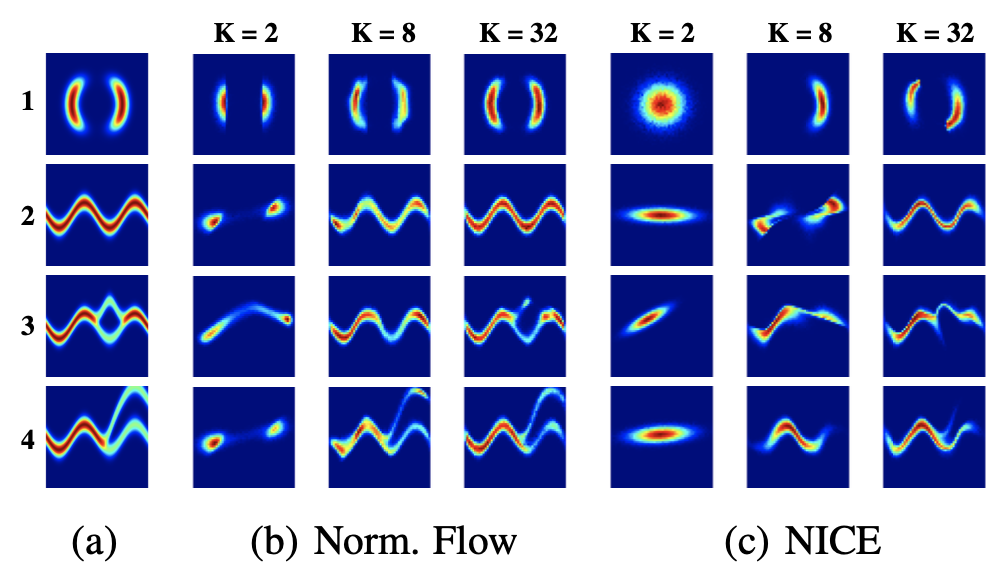
\includegraphics[width=0.9\columnwidth]{EFs}
      \end{center}
      
      \begin{block}{Experiments}
      \begin{itemize}
      	\item DLGM + NF
      	\item DLGM + NICE
      \end{itemize}
      
      \end{block}
      
      
	\begin{center}
        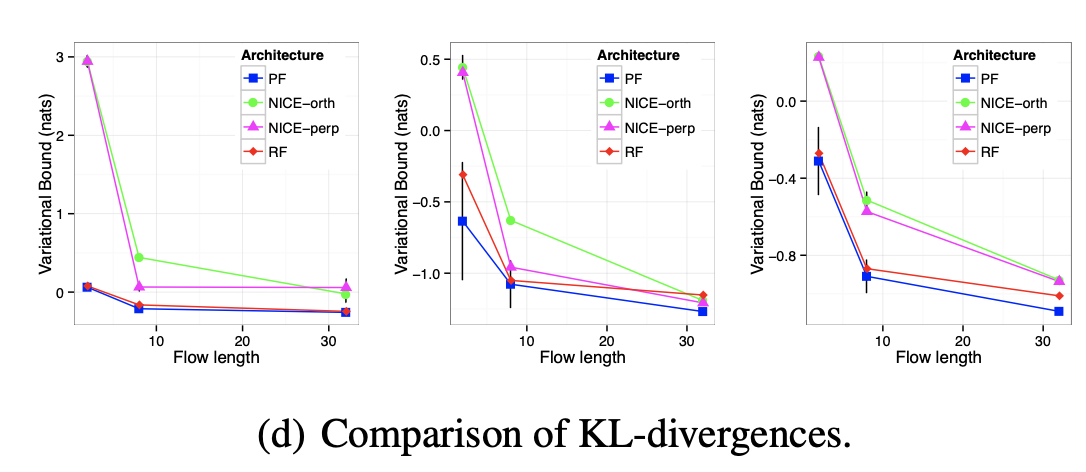
\includegraphics[width=0.9\columnwidth]{varbound}
      \end{center}

  \end{column} % End of the 2nd column
  

%%%%%%%%%%%%%%%%%%%%%%%%%%%%%%%%%%%%%%%%%%
%% Column 3
%%%%%%%%%%%%%%%%%%%%%%%%%%%%%%%%%%%%%%%%%%

  \begin{column}{.02\textwidth}\end{column} % Empty spacer column

  \begin{column}{.3\textwidth} % 3rd column

    \vspace{\shrink} 
    \begin{block}{Results}
        \textbf{TODO!!!}         
      Results...
    \end{block}
    
       \begin{center}
        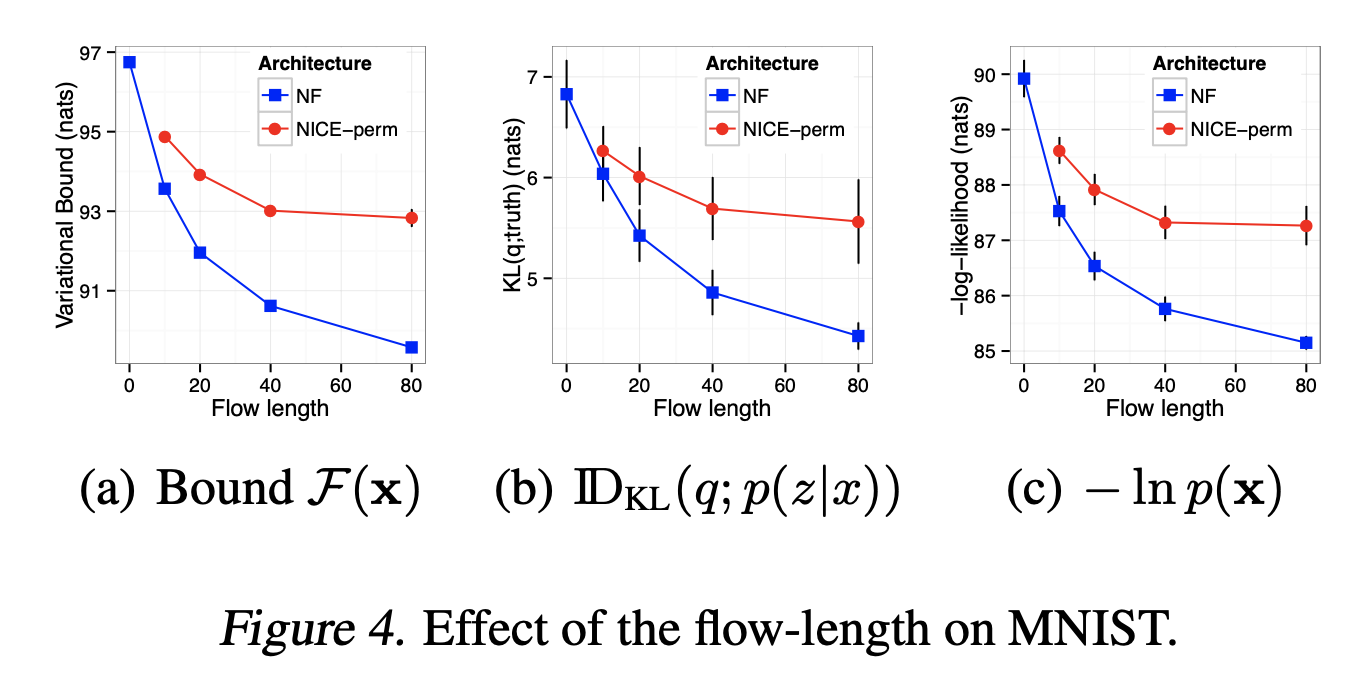
\includegraphics[width=0.9\columnwidth]{flowlen}
      \end{center}
    
    
    \begin{block}{Our Improvements and Extensions}
    
	\textbf{TODO} Pellentesque vitae dui velit. Aenean tincidunt eros facilisis turpis tincidunt, non mollis ipsum venenatis. Praesent consectetur venenatis est, quis rutrum justo faucibus vitae. Nam id orci ex. Aenean id finibus libero. Nam tristique pellentesque eros et mattis. Proin vel nunc accumsan, aliquet leo ut, consectetur sem. Ut ut elit libero. Donec aliquet nulla ac venenatis egestas. Maecenas eu nunc hendrerit turpis dictum laoreet at ut velit. Phasellus tempus tellus id leo bibendum, ac rhoncus turpis molestie. Quisque commodo, quam vitae elementum fermentum, erat dolor hendrerit quam, bibendum malesuada lectus lacus sit amet nisi. In dignissim nisl elit. Aenean vitae enim ut ligula congue vehicula sed non lacus.    
	
	\end{block}

    \begin{block}{References}
      \nocite{*} % Insert publications even if they are not cited in the poster
      \linespread{0.928}\selectfont
      \footnotesize{\bibliographystyle{unsrt}
      \bibliography{poster}}
    \end{block}

  \end{column} % End of the 3rd column

  \begin{column}{.02\textwidth}\end{column} % Empty spacer column

\end{columns} % End of all the columns in the poster

\end{frame} % End of the enclosing frame

\end{document}